\documentclass[11pt,aspectratio=169,handout]{beamer} 
\usetheme{Antibes} % si possono modificare in tutti i modi possibili
\usecolortheme{whale}
\usefonttheme[onlymath]{serif}

\definecolor{myTeal}{RGB}{31 122 140}
\definecolor{myMutedTeal}{RGB}{1 22 70}
\definecolor{myBlue}{RGB}{0 123 167}
\definecolor{myLavender}{RGB}{118 108 127}
\definecolor{myApricot}{RGB}{249 219 189}
%\definecolor{myGreen}{RGB}{34 139 34}
%\definecolor{myGreen}{RGB}{0 150 44}
%\definecolor{myGreen}{RGB}{37 110 75}
\definecolor{myGreen}{RGB}{19 96 55}
%\definecolor{myGreen}{RGB}{43 129 88}

\setbeamercolor{structure}{fg=myGreen} % bullet points
\setbeamercolor{palette primary}{bg=myGreen, fg=white} % headers colour
\setbeamercolor{titlelike}{fg=white} % titles colour 

\setbeamertemplate{navigation symbols}{} % nasconde i pulsanti di navigazione
\setbeamertemplate{headline}{} % navigazione in cima

\usepackage{appendixnumberbeamer}
\usepackage{mathtools}
\usepackage{lipsum}

% per l'handout
% \usepackage{pgfpages}
% \pgfpagesuselayout{4 on 1}[a4paper, border shrink = 5mm]

\usepackage[utf8]{inputenc}
\usepackage[italian]{babel}
\usepackage{caption}

\usepackage{chronosys}
\setupchronoevent{textwidth=3cm, textstyle=\centering}

\newtheorem{teo}[theorem]{Teorema}
\newtheorem{de}[theorem]{Definizione}
\newtheorem{no}[theorem]{Nota}
\setbeamercolor{block title}{bg=myGreen,fg=white} 

\newcommand{\COMMENT}[1]{} %comment block
\usepackage{amsmath,physics}

\title{\textbf{Metodi Supersimmetrici per la Meccanica Quantistica}}
\author{Paolo Rocchietti March \\ Relatrice: Marialuisa Frau}
\date{20 novembre 2026}

\begin{document}

\section{Intro}

\begin{frame}[plain] %Frames are slides
    \centering
    
\includegraphics[width=2cm]{logounito.png}\par
    \maketitle
\end{frame}

\setbeamertemplate{footline}{ % this sets the headers & footers
    \hspace{0.5cm}
    
\includegraphics[width=0.7cm]{logounito.png}
    \hfill%
    \usebeamercolor[fg]{page number in head/foot}%
    \usebeamerfont{page number in head/foot}%
    \insertframenumber\,/\,\inserttotalframenumber\kern1em\vskip2pt% pag/tot
}

%\setbeamertemplate{footline}{ % this sets the headers & footers
%  \hspace{0.5cm}
%  \usebeamercolor[fg]{page number in head/foot}%
%  \usebeamerfont{page number in head/foot}%
%  \insertframenumber\,/\,\inserttotalframenumber\kern1em\vskip0pt% pag/tot
%  \hfill%
%  
\includegraphics[width=0.7cm]{logounito.png}
%}

\begin{frame}{Indice} %title of the slide
    \begin{columns}       %columns
        \column{.55\textwidth}
        \begin{enumerate}
            \item Algebra di Supersimmetria.
                \vspace{0.3cm}
            \item Hamiltoniane \textit{partner} supersimmetriche:
                \begin{itemize}
                    \item Rapporto tra autostati e tra autovalori;
                    \item Spettri discreti;
                    \item Supersimmetria rotta e non rotta;
                    \item Esempio: la buca infinita di potenziale (?).
                \end{itemize}
        \end{enumerate}
        %\vspace{0.3cm}
        \column{.45\textwidth}
        \begin{enumerate}
            \setcounter{enumi}{2} 
            \item \textit{Shape invariance}:
                \begin{itemize}
                    \item Operatori scala generalizzati;
                    \item Esempio: l'oscillatore armonico isotropo.
                \end{itemize}
                \vspace{0.3cm}
            \item Metodo SWKB:
                \begin{itemize}
                    \item SWKB del primo ordine;
                    \item SWKB per potenziali \textit{shape invariant}.
                \end{itemize}
        \end{enumerate}
    \end{columns}
\end{frame}

\section{SUSY Algebra}

\begin{frame}{Algebra di Supersimmetria/1}
    Data una funzione reale $W(x)$, detta \textit{superpotenziale}, si considerano
    gli operatori
    $${A} :=  \frac{\hbar}{\sqrt{2m}}\dv[]{}{x}+W(x),\quad{A}^\dagger =
    -\frac{\hbar}{\sqrt{2m}}\dv[]{}{x}+W(x):$$
    da essi si definiscono due Hamiltoniane
    $$H_1 := A^\dagger A = -\frac{\hbar^2}{2m}\dv[2]{}{x} + V_1(x),\quad
    H_2:=AA^\dagger = -\frac{\hbar^2}{2m}\dv[2]{}{x}+V_2(x),$$
    dove
    $$V_1(x) = W^2(x) - \frac{\hbar}{\sqrt{2m}}W'(x),\quad V_2(x) = W^2(x) +
    \frac{\hbar}{\sqrt{2m}}W'(x).$$
\end{frame}

\begin{frame}{Algebra di Supersimmetria/2}
    Queste Hamiltoniane possono essere viste come elementi di una Hamiltoniana a
    blocchi $H$: definendo
    $$Q = \begin{pmatrix}
        \mathbb{O}&\mathbb{O}\\
        A&\mathbb{O}
        \end{pmatrix},\quad Q^\dagger=\begin{pmatrix}
        \mathbb{O}&A^\dagger\\
        \mathbb{O}&\mathbb{O}
    \end{pmatrix},
    $$
    si ha che
    $$H := \left\{Q,Q^\dagger\right\}=\begin{pmatrix}
        H_1&\mathbb{O}\\
        \mathbb{O}&H_2
    \end{pmatrix}.
    $$
    Per costruzione, gli operatori $Q,Q^\dagger,H$ soddisfano anche le relazioni
    $$\left[H,Q\right]=\left[H,Q^\dagger\right]=0,\quad
    \left\{Q,Q\right\}=\left\{Q^\dagger,Q^\dagger\right\}=0.
    $$
    Queste 5 relazioni definiscono la \textbf{superalgebra di Lie} $sl(1/1)$.

    È noto che l'esistenza di operatori commutanti
    con $H$ porti a \textbf{degenerazioni negli autostati di energia}:
    si vedrà in seguito come questo accade anche in questo caso.
\end{frame}
\begin{frame}[t]{Hamiltoniane \textit{partner} supersimmetriche}
    \begin{columns}
        \column{0.5\textwidth}
        \begin{de}
            Le Hamiltoniane nella forma
            $$H_1 = A^\dagger A,\; H_2 = AA^\dagger$$
            si definiscono \textit{partner supersimmetriche}.
        \end{de}
        La peculiarità di queste Hamiltoniane è che sono accomunate dalla scelta
        del superpotenziale $W(x)$, che ``genera'' i due potenziali $V_1(x)$ e $V_2(x)$.
        \column{0.5\textwidth}
        \phantom{miao}\\
        Vale inoltre il seguente teorema, di facile dimostrazione, sui loro autovalori
        di energia:
        \begin{teo}
            Due Hamiltoniane partner supersimmetriche presentano sempre spettro energetico
            semi-definito positivo, cioè
            $$H_i\ket{E^{(i)}} = E^{(i)}\ket{E^{(i)}},\;\text{con }E^{(i)}\geq0$$
        \end{teo} 
    \end{columns}
\end{frame}
\begin{frame}{Rapporto tra autostati e tra autovalori}
    La proprietà più importante delle Hamiltoniane supersimmetriche è che i loro
    autovalori e autostati associati sono legati tra loro.

    Considerando infatti un autostato $\ket{E^{(1)}}$ di $H_1$ con
    autovalore $E$
    $$H_1\ket{E^{(1)}}=E\ket{E^{(1)}}$$
    si applica l'operatore $A$ a sinistra, \textbf{supponendo}
    $\mathbf{A\ket{E^{(1)}}\neq0}$:
    $$\underbrace{AA^\dagger}_{:=H_2} A\ket{E^{(1)}}=EA\ket{E^{(1)}}
    \implies H_2\left(A\ket{E^{(1)}}\right) = E\left(A\ket{E^{(1)}}\right).$$
    Si trova che $\mathbf{A\ket{E^{(1)}}}$ \textbf{è un autostato di}
    $\mathbf{H_2}$ \textbf{con stesso autovalore}
    $\mathbf{E}$, a meno di normalizzazioni.
    Se invece $A\ket{E^{(1)}}=0$ si ha automaticamente che $E=0$.
\end{frame}



%\begin{frame}{Spettri discreti/1}
%    \begin{columns}
%       \column{.45\textwidth}
%       Nel caso in cui gli spettri delle Hamiltoniane siano discreti, si denota
%       $$H_i \psi_n^{(i)} = E_n^{(i)}\psi_n^{(i)}$$
%       e la relazione appena ricavata si scrive
%       $$\psi_n^{(2)} = A\psi_n^{(1)},\;\text{se }E^{(1)}_n\neq0.$$
%   Similmente si può mostrare che
%   $$\psi_n^{(1)} = A^\dagger\psi_n^{(2)},\;\text{se }E^{(2)}_n\neq0$$
%   \column{.55\textwidth}
%   Nel caso in cui l'autovalore $E^{(i)}_n$ sia nullo, lo stato a esso associato
%   è sicuramente lo stato fondamentale di $H_i$ e vale, rispettivamente, che
%   $$A\psi_0^{(1)} = 0,\;A^\dagger\psi_0^{(2)}=0.$$
%   Esplicitando la forma degli operatori, queste condizioni sono equazioni
%   differenziali da cui si possono ricavare le autofunzioni $\psi^{(i)}_0(x)$
%   a partire dal superpotenziale $W(x)$:
%   \begin{gather*}
%   \psi^{(1)}_0(x)=N\exp\left[-\frac{\sqrt{2m}}{\hbar}\int_{x_0}^{x}\dd y
%   W(y)\right]\\
%   \psi^{(2)}_0(x)=N\exp\left[\frac{\sqrt{2m}}{\hbar}\int_{x_0}^{x}\dd y
%   W(y)\right].
%   \end{gather*}
%   \end{columns} 
%\end{frame}



\begin{frame}{Spettri discreti/1}
    Nel caso in cui gli spettri delle Hamiltoniane siano discreti, si denota
    $$H_i \psi_n^{(i)} = E_n^{(i)}\psi_n^{(i)}$$
    e la relazione appena ricavata si scrive
    $$\ket{E^{(2)}} = A\ket{E^{(1)}}\longrightarrow \boxed{\psi_n^{(2)} =
    A\psi_n^{(1)},\;\text{se }E^{(1)}_n\neq0.}$$
    Similmente si può mostrare che
    $$\ket{E^{(1)}} = A^\dagger\ket{E^{(2)}}\longrightarrow\boxed{\psi_n^{(1)}
    = A^\dagger\psi_n^{(2)},\;\text{se }E^{(2)}_n\neq0}$$
    Nel caso in cui l'autovalore $E^{(i)}_n$ sia nullo, lo stato a esso associato
    è sicuramente lo stato fondamentale di $H_i$ e vale, rispettivamente, che
    $$A\psi_0^{(1)} = 0,\;A^\dagger\psi_0^{(2)}=0.$$
\end{frame}
\begin{frame}{Spettri discreti/2}
    Esplicitando la forma degli operatori, queste condizioni sono equazioni
    differenziali da cui si possono ricavare le autofunzioni $\psi^{(i)}_0(x)$
    a partire dal superpotenziale $W(x)$:
    \begin{gather*}
        \psi^{(1)}_0(x)=N\exp\left[-\frac{\sqrt{2m}}{\hbar}\int_{x_0}^{x}\dd y
        W(y)\right]\\
        \psi^{(2)}_0(x)=N\exp\left[\frac{\sqrt{2m}}{\hbar}\int_{x_0}^{x}\dd y
        W(y)\right].
    \end{gather*}
    \begin{teo}
        Solo una delle due Hamiltoniane partner può avere autovalore $E=0$:
        \begin{gather*}
            E_0^{(1)}=0\implies E_0^{(2)}\neq 0,\quad
            E_0^{(2)}=0\implies E_0^{(1)}\neq 0
        \end{gather*}
    \end{teo}
\end{frame}
\begin{frame}{Spettri discreti/3}
    La convenzione adottata nella letteratura è che $W(x)$ sia scelto in modo
    che \textbf{al più} $H_1$ presenti uno stato con autovalore di energia nullo.\\
    \phantom{miao}

    La condizione $A\psi^{(1)}_0 = 0$, nel caso in cui si conosca la funzione
    d'onda dello stato fondamentale, fornisce anche un'espressione per il
    superpotenziale (sempre ottenuta esplicitando l'operatore $A$):
    $$
    W(x)=-\frac{\hbar}{\sqrt{2m}}\frac{\psi'^{(1)}_0(x)}{\psi^{(1)}_0(x)}.
    $$
    Essa sarà utile in seguito per ricavare il superpotenziale associato a
    potenziali conosciuti per risolverne di nuovi.
\end{frame}

\begin{frame}{Supersimmetria rotta e non rotta/1}
    \begin{columns}[t]
        \column{.5\textwidth}
        \begin{de}
            La Supersimmetria si dice \textbf{spontaneamente rotta} se e solo se
            $$A\psi^{(1)}_0\neq0.$$
        \end{de}
        \begin{de}
            La Supersimmetria si dice \textbf{non rotta} se e solo se
            $$A\psi^{(1)}_0 = 0,$$
        \end{de}
        \column{.5\textwidth}
        La supersimmetria è dunque \textbf{non rotta} se $\mathbf{E_0^{(1)}=0}$.\\
        \phantom{miao}\\
        In entrambi i casi, oltre al legame tra le autofunzioni sopra esplicitato,
        gli autovalori non nulli sono a due a due uguali:
        poiché si denota sempre con $n=0$ lo stato fondamentale, i pedici degli autovalori
        saranno diversi per Supersimmetria non rotta e spontaneamente rotta.
        $$E^{(1)}_0 = 0 \implies E^{(1)}_{n+1} = E^{(2)}_n,\;\forall n = 0,1,2...$$
        $$E^{(1)}_0\neq0\implies E^{(1)}_n = E^{(2)}_n,\;\forall n=0,1,2...$$
    \end{columns}
\end{frame}
\begin{frame}{Supersimmetria rotta e non rotta/2}
    Le definizioni appena fornite possono essere riscritte in termini
    degli operatori della superalgebra $Q,Q^\dagger$: sia
    $$\psi_0:=\begin{pmatrix}
        \psi_0^{(1)}\\\psi_0^{(2)}
    \end{pmatrix}
    $$
    lo stato fondamentale dell'Hamiltoniana $H$, allora la condizione di
    Supersimmetria non rotta implica
    $$
    \begin{dcases}
        A\psi^{(1)}_0 = 0\\
        \psi_0^{(2)}\equiv0
    \end{dcases} 
    \iff
    \begin{dcases}
        Q\psi_0 = \begin{pmatrix}
            \mathbb{O}&\mathbb{O}\\
            A&\mathbb{O}
            \end{pmatrix}\begin{pmatrix}
            \psi^{(1)}_0\\ 0
        \end{pmatrix} = 0 \\
        Q^\dagger\psi_0 = \begin{pmatrix}
            \mathbb{O}&A^\dagger\\
            \mathbb{O}&\mathbb{O}
            \end{pmatrix}\begin{pmatrix}
            \psi^{(1)}_0\\ 0
        \end{pmatrix} = 0
    \end{dcases}.
    $$
    Da questa definizione equivalente è chiaro che l'espressione ``rottura spontanea''
    sia utilizzata in parallelismo alla definizione di rottura spontanea di
    simmetria.

\end{frame}

\begin{frame}{Supersimmetria rotta e non rotta/3}
    \begin{figure}[H]
        \centering
        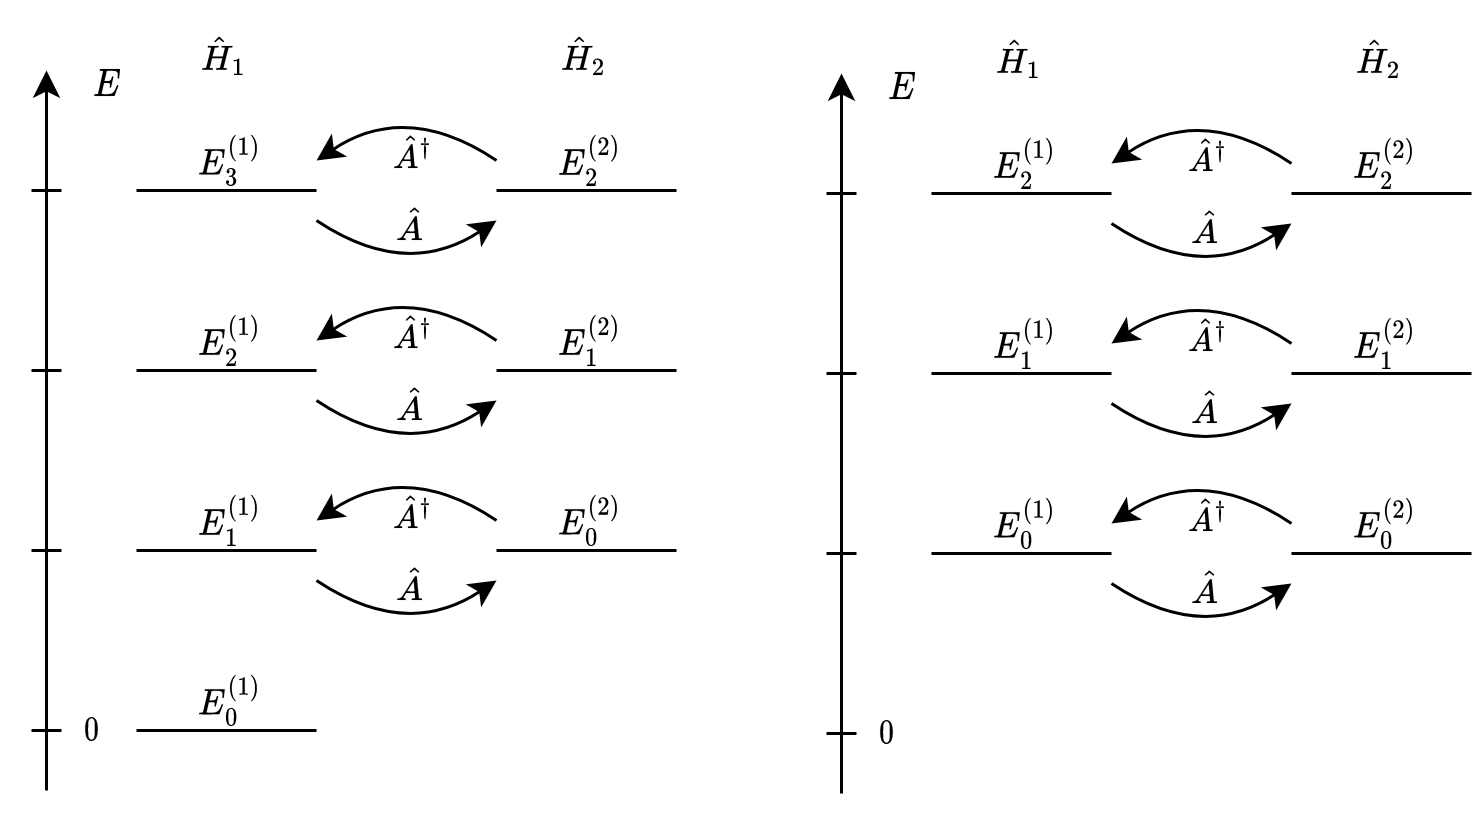
\includegraphics[width = .75\linewidth]{./SUSY_levels.png}
        \caption{\footnotesize Diagramma riassuntivo dello spettro discreto
            di due Hamiltoniane \textit{partner}, con supersimmetria non rotta (sinistra)
        e spontaneamente rotta (destra).}
    \end{figure}
\end{frame}
\begin{frame}{Esempio: la buca infinita di potenziale (?)/1}
    Si consideri la buca infinita di potenziale, con un \textit{offset} energetico
    tale da rendere lo stato fondamentale a energia nulla:
    $$V_1(x)=\begin{dcases}
        -\frac{\pi^2\hbar^2}{2mL^2}&\text{se } 0\leq x\leq L\\
        \infty&\text{altrimenti}
    \end{dcases},
    $$
    i cui autovalori e autofunzioni sono ben noti
    $$
    E^{(1)}_n = \frac{\pi^2\hbar^2}{2mL^2}n(n+2),\quad
    \psi^{(1)}_n(x)=\sqrt{\frac{2}{L}}\sin\left(\frac{(n+1)\pi x}{L}\right),\;
    \text{con }n=0,1,2,3...$$
    Come esplicitato in precedenza, dallo stato fondamentale si può ricavare il
    superpotenziale corrispondente a $V_1$:
    $$W(x) = -\frac{\hbar}{\sqrt{2m}}\frac{\psi'^{(1)}_0(x)}{\psi_0^{(1)}(x)} = 
    -\frac{\hbar\pi}{L\sqrt{2m}}\cot\left(\frac{\pi x}{L}\right).
    $$
\end{frame}
\begin{frame}{Esempio: la buca infinita di potenziale (?)/2}
    Il potenziale $V_2$, \textit{partner} di $V_1$, può essere ricavato da $W(x)$
    $$V_2(x)=W^2(x)+\frac{\hbar}{\sqrt{2m}}W'(x)=
    \frac{\pi^2\hbar^2}{2mL^2}\left[2\sin^{-2}\left(\frac{\pi x}{L}\right)-1\right]$$
    e, per le proprietà sopra citate della Supersimmetria non rotta, il suo spettro
    energetico è semplicemente
    $$E^{(2)}_n=E^{(1)}_{n+1}=\frac{\pi^2\hbar^2}{2mL^2}(n+1)(n+3)\;
    \text{con }n=0,1,2,3...$$
    L'autofunzione dello stato fondamentale di $V_2(x)$ si può ricavare, a meno di
    normalizzazioni, da $\psi^{(1)}_1(x)$ utilizzando l'espressione esplicita di $A$:
    $$\psi^{(2)}_0(x)=A\psi_1^{(1)}(x) = \sin^2\left(\frac{\pi x}{L}\right)$$
    e similmente tutte le altre.
\end{frame}
\begin{frame}{\textit{Shape Invariance}}
    \phantom{\small miao}
    \begin{columns}[t]
        \column{.5\linewidth}
        Considerando un superpotenziale $W(x;a_1)$ dipendente da un insieme di
        parametri $a_1$
        si costruiscono due potenziali \textit{partner} supersimmetrici
        $V_1(x;a_1),V_2(x,a_1)$ anch'essi dipendenti dai parametri $a_1$.
        \begin{de}
            Due potenziali partner supersimmetrici $V_1,V_2$ si dicono shape invariant se
            e solo se
            $$V_2(x;a_1) = V_1(x;a_2) + R(a_1)$$
            dove $a_2=f(a_1)$ e $R(a_1)$ non dipende da $x$.
        \end{de}
        %Intuitivamente, due potenziali sono shape invariant se i loro parametri
        %sono gli uni in funzione degli altri e se differiscono per un offset energetico
        %costante dipendente dai parametri.
        \column{.5\linewidth}
        Si ha dunque che
        $$H_2(a_1) = H_1(a_2)+R(a_1)$$
        dunque gli spettri energetici differiscono per una costante
        $$E_n^{(2)}(a_1)=E^{(1)}_n(a_2)+R(a_1)$$
        e le autofunzioni sono le medesime
        $$\psi_0^{(2)}(x;a_1) = \psi^{(1)}_0(x;a_2)$$
        a meno di normalizzazioni e della funzione $f$ applicata sui parametri, che è
        nota.
    \end{columns}
\end{frame}
\begin{frame}{Operatori scala generalizzati/1}
    \begin{columns}
        \column{0.5\linewidth}
        Ricordando che $H_1,H_2$ sono \textit{partner} supersimmetriche, vale la
        relazione
        $$\psi_1^{(1)}(x;a_1) = A^\dagger(a_1)\psi^{(2)}_0(x;a_1)$$
        dunque, per la proprietà di \textit{shape invariance},
        $$\psi_1^{(1)}(x;a_1)=A^\dagger(a_1)\psi^{(1)}_0(x;a_2)$$
        Questo processo può essere generalizzato per costruire \textit{tutti} gli stati
        eccitati di $H_1(a_1)$ a partire dallo stato fondamentale.
        \column{0.5\linewidth}
        \begin{teo}
            Data la famiglia di potenziali
            $$V_s(x;a_1) = V_1(x;a_s)+\sum_{k=1}^{s-1}R(a_k)$$
            dove $a_k=f^{k-1}(a_1)$, i potenziali
            $$V_i(x;a_1),\;V_{i+1}(x;a_1)$$
            sono partner supersimmetrici e shape invariant $\forall i =1,2...$.
        \end{teo} 
    \end{columns}
\end{frame}
\begin{frame}{Operatori scala generalizzati/2}
    %\begin{columns}
    %  \column{0.5\textwidth}
    Se la Supersimmetria è non rotta, lo spettro energetico di $H_1(a_1)$ è
    facilmente calcolabile: infatti
    $$E_1^{(1)}(a_1) = E_0^{(2)}(a_2) = E_0^{(1)}+R(a_1)=R(a_1)$$
    similmente il livello successivo vale
    \begin{gather*}
        E_2^{(1)}(a_1) = E^{(2)}_1(a_1)=E^{(3)}_0(a_1)
        = E_0^{(2)}(a_2)+R(a_1) = R(a_1)+R(a_2)
    \end{gather*}
    e, iterando, l'$n-$esimo
    $$E^{(1)}_n(a_1)=\sum_{k=1}^{n}R(a_k)$$
    che è anche l'energia dello stato fondamentale di $H_{n+1}(a_1)$:
    $$E_0^{(n+1)} = E_n^{(1)}(a_1)$$
    poiché $H_s$ sono tutte \textit{partner}.
    %  \column{0.5\textwidth}
    %\end{columns}

\end{frame}

\begin{frame}{Operatori scala generalizzati/3}
    Definendo gli operatori
    $$A_s := A(a_s),\;A^\dagger_s:=A^\dagger(a_s)$$
    che agiscono tra $H_s$ e $H_{s+1}$ come $A,A^\dagger$ agiscono su
    $H_1$ e $H_2$, per determinare le autofunzioni vale un procedimento simile:
    l'autofunzione del primo stato eccitato è
    $$\psi_1^{(1)}(x;a_1) = A_1^\dagger\psi_0^{(2)}(x;a_1) = A_1^\dagger
    \psi_0^{(1)}(x;a_2)$$
    quella del secondo è
    $$\psi_2^{(1)}(x;a_1) = A^\dagger_1A^\dagger_2\psi_0^{(3)}(x;a_1)$$
    Applicando due volte la \textit{shape invariance}
    $$\psi_2^{(1)}(x;a_1)= A_1^\dagger A_2^\dagger\psi_0^{(1)}(x;a_3).$$
    Iterando questo processo si ottiene che l'$n-$esima autofunzione vale
    $$\psi_n^{(1)}(x;a_1)=A_1^\dagger \psi_{n-1}^{(1)}(x;a_2)=
    A_1^\dagger...A_n^\dagger\psi^{(1)}_0(x;a_{n+1})
    $$
\end{frame}
\begin{frame}{Operatori scala generalizzati/4}
    \begin{figure}[H]
        \centering
        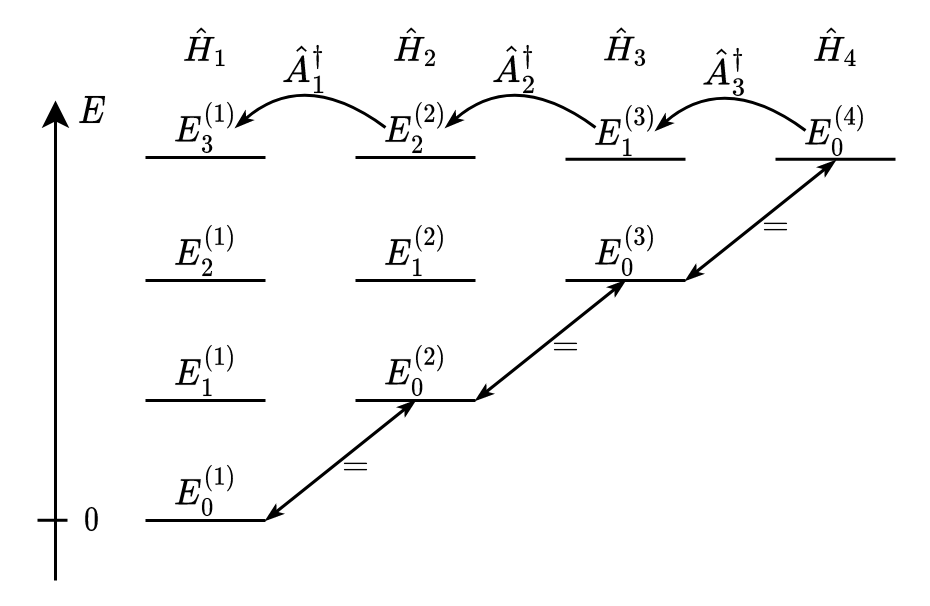
\includegraphics[width = .7\linewidth]{./shape_inv.png}
        \caption{\footnotesize Diagramma per la costruzione del terzo stato eccitato
        di $H_1(a_1)$.}
    \end{figure}
\end{frame}
\begin{frame}{Esempio: l'oscillatore armonico isotropo/1}
    Tutte le considerazioni precedenti sono valide anche per potenziali radiali
    nelle equazioni di Schrödinger radiali ridotte: ponendo 
    $\hbar = 2m = 1$, si consideri il superpotenziale
    $$W(r;l)=\frac{\omega r}{2}-\frac{l+1}{r},$$
    a cui sono associati i due potenziali \textit{partner}
    \begin{equation*}
        \begin{dcases}
            V_1(r;l)=\frac{\omega^2r^2}{4}+\frac{l(l+1)}{r^2}-\left(l+\frac{3}{2}\right)\omega\\
            V_2(r;l)=\frac{\omega^2r^2}{4}+\frac{(l+1)(l+2)}{r^2}-\left(l+\frac{1}{2}\right)
            \omega
        \end{dcases}:
    \end{equation*}
    è facile mostrare che sono \textit{shape invariant}, infatti
    $$V_2(r;l) = V_1(r;l+1)+2\omega,$$
    con $a_2:=f(a_1=l)=l+1$ e $R(a_1=l)=2\omega$.
\end{frame}
\begin{frame}{Esempio: l'oscillatore armonico isotropo/2}
    La supersimmetria è non rotta, infatti la funzione d'onda radiale ridotta dello
    stato fondamentale
    $$R_0^{(1)}(r;l) = \exp\left[-\int_{r_0>0}^r \dd \rho \frac{\omega\rho}{2}
    -\frac{l+1}{\rho}\right] = r^{l+1}e^{-\frac{\omega}{4}r^2}$$
    è normalizzabile. Dalle proprietà della \textit{shape invariance} appena ricavate
    si può determinare lo spettro energetico
    $$E_n^{(1)}(l)=\sum_{k=1}^{n}R(a_k)=\sum_{k=1}^{n}2\omega = 2n\omega$$
    e, ricorsivamente, tutte le funzioni d'onda radiali ridotte: la prima è
    $$R_1^{(1)}(r;l)=A^\dagger(l)R_0^{(1)}(r;l+1)=(\omega r^2-2l-3)r^{l+1}
    e^{-\frac{\omega}{4}r^2}.$$
\end{frame}
\begin{frame}{Esempio: l'oscillatore armonico isotropo/3}
    \begin{columns}
        \column{.55\textwidth}
        Per la teoria generale sui potenziali radiali, le autofunzioni complete sono
        \begin{align*}
    &\psi^{(1)}_{0lm}(r,\vartheta,\varphi) = r^le^{-\frac{\omega}{4}r^2}Y_{lm}
    (\vartheta,\varphi)\\
    &\psi_{1lm}(r,\vartheta,\varphi) = (\omega r^2-2l-3)r^{l}e^
    {-\frac{\omega}{4}r^2}Y_{lm}(\vartheta,\varphi).
        \end{align*}
        \begin{no}
            Il numero quantico $n$ qui utilizzato non è il medesimo utilizzato nella
            trattazione dell'oscillatore armonico isotropo su molti testi di Meccanica
            Quantistica: esso corrisponde a $N = 2n+l$. 
        \end{no}
        \column{.45\textwidth}
        Queste due autofunzioni sono esattamente quelle che si ricavano risolvendo
        analiticamente il problema: si nota infatti che
        $$(\omega r^2 - 2l - 3)\propto L_{1}^{\left(l+\frac{1}{2}\right)}\left(
        \frac{\omega}{2}r^2\right)$$
        dove $L_k^{(\alpha)}(x)$ sono i polinomi generalizzati di Laguerre.

        Questo esempio evidenzia come un problema con una soluzione analitica non
        banale possa essere risolto molto semplicemente utilizzando l'algebra di 
        Supersimmetria.
    \end{columns}
\end{frame}


\begin{frame}{Metodo SWKB}
    \begin{columns}
        \column{.5\textwidth}
        Un'altra applicazione della Supersimmetria in Meccanica Quantistica è il
        metodo SWKB, una variante supersimmetrica dell'approssimazione WKB. 
        \begin{figure}[H]
            \centering
            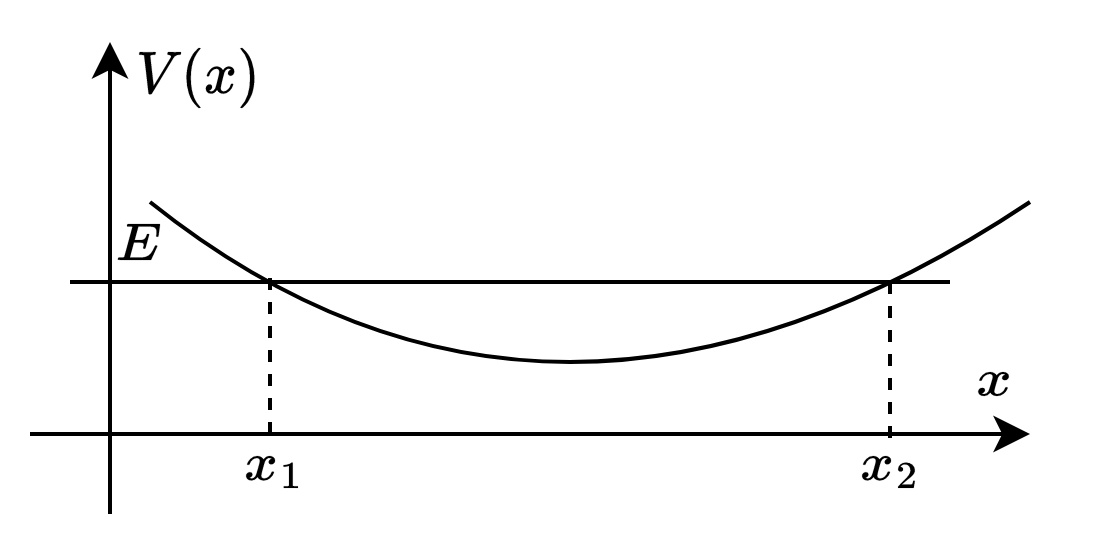
\includegraphics[width = .8\linewidth]{./gen_well.png}
            \caption{\footnotesize Buca di potenziale generalizzata, con $V(x_1)=
            V(x_2)=E$.}
        \end{figure}
        \column{.5\textwidth}
        In particolare, è noto che, data una buca di potenziale generalizzata $V(x)$
        e un valore di energia $E$ come in figura, dal WKB di primo ordine si può
        ricavare la condizione di quantizzazione dell'energia
        \begin{equation*}
            \int_{x_1}^{x_2}\dd y \sqrt{2m\left[E_n-V(y)\right]}=\left(n+\frac{1}{2}\right)
            \hbar\pi,
        \end{equation*}
        che è un'approssimazione del valore di $E_n$ che migliora all'aumentare di
        $n$.

        Per potenziali \textit{partner} supersimmetrici si può ulteriormente
        migliorare l'approssimazione.
    \end{columns}

\end{frame}
\begin{frame}{SWKB del primo ordine/1}
Il nucleo di questo miglioramento si trova nel fatto che \textbf{i potenziali
\textit{partner} hanno una dipendenza $O(\hbar)$ esplicita} (supponendo
$W(x)=O(\hbar)$) che può essere tolta dall'integrale.
La condizione di quantizzazione per $V_1$ è
$$
\int_{x_1}^{x_2}\dd y \sqrt{2m\left[E^{(1)}_n-W^2(y)+\frac{\hbar}{\sqrt{2m}}W'(y)
\right]}
=\left(n+\frac{1}{2}\right)\hbar\pi:
$$
lo sviluppo in potenze di $\hbar$ dell'integrando è
$$\sqrt{2m\left(E_n^{(1)}-W^2(y)\right)}+\frac{\hbar}{2}\frac{W'(y)}
{\sqrt{E_n^{(1)}-W^2(y)}}+O(\hbar^2),$$
mentre gli estremi di integrazione sono ridefiniti in modo che
$$W^2(a)=W^2(b)=E_n^{(1)}.$$

\end{frame}

\begin{frame}{SWKB del primo ordine/2}
Il termine $O(\hbar)$ può essere integrato esplicitamente:
$$\int_{a}^{b} \dd y \frac{W'(y)}{\sqrt{E_n^{(1)}-W^2(y)}} = \eval{
\arcsin\left(\frac{W(y)}{\sqrt{E_n^{(1)}}}\right)}_a^b.$$
Nel caso di \textbf{supersimmetria non rotta}, la normalizzabilità di
$\psi_0^{(1)}$ implica che il superpotenziale debba avere segni opposti nei limiti
a $\pm\infty$, quindi $$-\sqrt{W(a)}=\sqrt{W(b)}=\sqrt{E_n^{(1)}}$$ e la condizione
di quantizzazione risulta
$$\int_{x_1}^{x_2} \dd y\sqrt{2m\left(E_n^{(1)}-W^2(y)\right)}=n\hbar\pi.$$
Questa condizione è \textbf{esatta per $\mathbf{n=0}$}, in quanto $a=b$ e dunque
$E_0^{(1)}=0$.
\end{frame}



\begin{frame}{SWKB e \textit{shape invariance}}
    \begin{columns}[t]
        \column{0.55\textwidth}
        Per i potenziali \textit{shape invariant} la condizione SWKB è ancora
        più potente: considerando la famiglia di potenziali $V_s$ definita in
        precedenza, ricordando che
        $$E^{(1)}_n = E_n^{(s)}-\sum_{k=1}^{s-1}R(a_k)$$
        la condizione SWKB $E_0^{(1)}=0$ per $V_1$ diventa
        $$E_0^{(s)}=\sum_{k=1}^{s-1}R(a_k).$$
        \column{0.45\textwidth}
        Visto che i potenziali $V_s$ sono \textbf{tutti \textit{partner}}, i livelli
        energetici sono i medesimi, in particolare
        $$E_0^{(n+1)} = E_n^{(1)}.$$
        Visto che tutti gli stati fondamentali $E^{(s)}_0$ sono esattamente
        determinati dal primo ordine del SWKB, questa relazione implica che
        \textbf{per potenziali \textit{shape invariant} gli autovalori di energia
        sono tutti esatti al primo ordine.}
    \end{columns}

\end{frame}









\section{Conclusioni}

\begin{frame}{Conclusioni}
\COMMENT{    \begin{columns}
        \column{0.6\textwidth}
        \vspace{-0.3cm}
        \begin{enumerate}
            \item i settori perturbativi e non-perturbativi sono legati tra loro dalla struttura analitica delle trans-serie
            \item esistono metodi numerici per ricostruire i settori non-perturbativi da un numero limitato di coefficienti perturbativi
            \item il metodo WKB esatto fornisce un framework per risolvere \emph{``esattamente''} problemi in meccanica quantistica
        \end{enumerate}
        \column{0.4\textwidth}
        \!\!\!``For the most part, it is true that the results [found using divergent series] are correct, which is very strange. \\ I am working to find out why, a \textcolor{myTeal}{very interesting problem}.''

        \vspace{0.1cm}
        \hrule

        \flushright continuing from Abel
\end{columns}}
\end{frame}


\appendix

\setbeamertemplate{footline}{
    \hspace{0.5cm}
    
\includegraphics[width=0.7cm]{logounito.png}
    \hfill%
}

\section*{Thank you!}

\begin{frame}[plain]
    \centering \Large
    \vspace{1.5cm}

    Grazie per l'attenzione!

    \vspace{1cm}

    
\includegraphics[width=2cm]{logounito.png}
\end{frame}

\section*{Backups}

%\begin{frame}{Metodo del punto a sella per Ai}

%\end{frame}

%\begin{frame}{Linea del tempo}
%\vspace{1cm}
%\startchronology[startyear=1830,stopyear=2026,height=0.5ex]
%\chronoevent[markdepth=50pt,vpos=100pt]{1841}{Stokes}
%\chronoevent[]{1838}{Airy}
%\chronoevent[]{1899}{Borel}
%\chronoevent[markdepth=50pt]{1926}{WKB}
%\chronoevent[markdepth=100pt]{1983}{Voros}
%\chronoevent[markdepth=50pt]{1981}{\'Ecalle}
%\chronoevent[]{1969}{Bender \& Wu}
%\chronoevent[date=false]{2020}{matrix models \\ renormalons \\ path integrals \\ strings}
%\stopchronology
%\end{frame}
\end{document}

